\chapter{Averaging systems}


\begin{description}
    \item[Distributed algorithm] \marginnote{Distributed algorithm}
        Given a network of $N$ agents that communicate according to a (fixed) digraph $G$ (each agent receives messages from its in-neighbors), a distributed algorithm computes:
        \[ x_i^{k+1} = \stf_i(x_i^k, \{ x_j^k \}_{j \in \mathcal{N}_i^\text{IN}}) \quad \forall i \in \{ 1, \dots, N \} \]
        where $x_i^k$ is the state of agent $i$ at time $k$ and $\stf_i$ is a local state transition function that depends on the current input states.

        \begin{remark}
            Out-neighbors can also be used.
        \end{remark}

        \begin{remark}
            If all nodes have a self-loop, the notation can be compacted as:
            \[ 
            x_i^{k+1} = \stf_i(\{ x_j \}_{j \in \mathcal{N}_i^\text{IN}}) 
            \quad
            \text{or}
            \quad
            x_i^{k+1} = \stf_i(\{ x_j \}_{j \in \mathcal{N}_i^\text{OUT}})
            \]
        \end{remark}
\end{description}



\section{Discrete-time averaging algorithm}

\begin{description}
    \item[Linear averaging distributed algorithm (in-neighbors)] \marginnote{Linear averaging distributed algorithm (in-neighbors)}
        Given the communication digraph with self-loops $G^\text{comm} = (I, E)$ (i.e., $(j, i) \in E$ indicates that $j$ sends messages to $i$), a linear averaging distributed algorithm is defined as:
        \[ x_i^{k+1} = \sum_{j \in \mathcal{N}_i^\text{IN}} a_{ij} x_j^k \quad i \in \{1, \dots, N\} \]
        where $a_{ij} > 0$ is the weight of the edge $(j, i) \in E$.

        \begin{description}
            \item[Linear time-invariant (LTI) autonomous system] \marginnote{Linear time-invariant (LTI) autonomous system}
                By defining $a_{ij} = 0$ for $(j, i) \notin E$, the formulation becomes:
                \[ x_i^{k+1} = \sum_{j=1}^N a_{ij} x_j^k  \quad i \in \{ 1, \dots, N \} \]

                In matrix form, it becomes:
                \[ \vec{x}^{k+1} = \matr{A}^T \vec{x}^k \]
                where $\matr{A}$ is the adjacency matrix of $G^\text{comm}$.

                \begin{remark}
                    This model is inconsistent with respect to graph theory as weights are inverted (i.e., $a_{ij}$ refers to the edge $(j, i)$).
                \end{remark}
        \end{description}

    \item[Linear averaging distributed algorithm (out-neighbors)] \marginnote{Linear averaging distributed algorithm (out-neighbors)}
        Given a fixed sensing digraph with self-loops $G^\text{sens} = (I, E)$ (i.e., $(i, j) \in E$ indicates that $j$ sends messages to $i$), the algorithm is defined as:
        \[ x_i^{k+1} = \sum_{j \in \mathcal{N}_i^\text{OUT}} a_{ij} x_j^k = \sum_{j=1}^{N} a_{ij} x_j^k \]
        In matrix form, it becomes:
        \[ \vec{x}^{k+1} = \matr{A} \vec{x}^k \]
        where $\matr{A}$ is the weighted adjacency matrix of $G^\text{sens}$.
\end{description}


\subsection{Stochastic matrices}

\begin{description}
    \item[Row stochastic] \marginnote{Row stochastic}
        Given a square matrix $\matr{A}$, it is row stochastic if its rows sum to 1:
        \[ \matr{A}\vec{1} = \vec{1} \]

    \item[Column stochastic] \marginnote{Column stochastic}
        Given a square matrix $\matr{A}$, it is column stochastic if its columns sum to 1:
        \[ \matr{A}^T\vec{1} = \vec{1} \]

    \item[Doubly stochastic] \marginnote{Doubly stochastic}
        Given a square matrix $\matr{A}$, it is doubly stochastic if it is both row and column stochastic.
\end{description}

\begin{lemma}
    An adjacency matrix $\matr{A}$ is doubly stochastic if it is row stochastic and the graph $G$ associated to it is weight balanced and has positive weights.
\end{lemma}

\begin{lemma} \phantomsection\label{th:strongly_connected_eigenvalues}
    Given a digraph $G$ with adjacency matrix $\matr{A}$, if $G$ is strongly connected and aperiodic, and $\matr{A}$ is row stochastic, its eigenvalues are such that:
    \begin{itemize}
        \item $\lambda = 1$ is a simple eigenvalue (i.e., algebraic multiplicity of 1),
        \item All others $\mu$ are $|\mu| < 1$.
    \end{itemize}

    \indenttbox
    \begin{remark}
        For the lemma to hold, it is necessary and sufficient that $G$ contains a globally reachable node and the subgraph of globally reachable nodes is aperiodic.
    \end{remark}
\end{lemma}


\subsection{Consensus}

\begin{theorem}[Discrete-time consensus] \marginnote{Discrete-time consensus}
    Consider a discrete-time averaging system with digraph $G$ and weighted adjacency matrix $\matr{A}$. Assume $G$ strongly connected and aperiodic, and $\matr{A}$ row stochastic. 
    
    It holds that there exists a left eigenvector $\vec{w} \in \mathbb{R}^N$, $\vec{w} > 0$ such that the consensus converges to:
        \[ 
            \lim_{k \rightarrow \infty} \vec{x}^k 
            = \vec{1}\frac{\vec{w}^T \vec{x}^0}{\vec{w}^T\vec{1}} 
            = \begin{bmatrix} 1 \\ \vdots \\ 1 \end{bmatrix} \frac{\sum_{i=1}^N w_i x_i^0}{\sum_{j=1}^N w_j}
            = \begin{bmatrix} 1 \\ \vdots \\ 1 \end{bmatrix} \sum_{i=1}^N \frac{w_i}{\sum_{j=1}^N w_j} x_i^0
        \]
        where $\tilde{w}_i = \frac{w_i}{\sum_{i=j}^N w_j}$ are all normalized and sum to 1 (i.e., they produce a convex combination).

    Moreover, if $\matr{A}$ is doubly stochastic, then it holds that the consensus is the average as $\vec{w} = 1$:
    \[ 
        \lim_{k \rightarrow \infty} \vec{x}^k = \vec{1} \frac{1}{N} \sum_{i=1}^N x_i^0
    \]

    % \begin{proof}[Sketch of proof]
    %     Let $\matr{T} = \begin{bmatrix} \vec{1} & \vec{v}^2 & \cdots & \vec{v}^N \end{bmatrix}$ be a change in coordinates that transforms an adjacency matrix into its Jordan form $\matr{J}$:
    %     \[ \matr{J} = \matr{T}^{-1} \matr{A} \matr{T} \]
    %     As $\lambda=1$ is a simple eigenvalue (\Cref{th:strongly_connected_eigenvalues}), it holds that:
    %     \[
    %         \matr{J} = \begin{bmatrix}
    %             1 & 0 & \cdots & 0 \\
    %             0 & & &  \\
    %             \vdots & & \matr{J}_2 &  \\
    %             0 & & &  \\
    %         \end{bmatrix}
    %     \]
    %     where the eigenvalues of $\matr{J}_2 \in \mathbb{R}^{(N-1) \times (N-1)}$ lie inside the open unit disk.

    %     Let $\vec{x}^k = \matr{T}\bar{\vec{x}}^k$, then we have that:
    %     \[
    %         \begin{split}
    %             &\vec{x}^{k+1} = \matr{A} \vec{x}^{k} \\
    %             &\iff \matr{T} \bar{\vec{x}}^{k+1} = \matr{A} (\matr{T} \bar{\vec{x}}^k) \\
    %             &\iff \bar{\vec{x}}^{k+1} = \matr{T}^{-1} \matr{A} (\matr{T} \bar{\vec{x}}^k) = \matr{J}\bar{\vec{x}}^k 
    %         \end{split}
    %     \]
    %     Therefore:
    %     \[
    %         \begin{gathered}
    %             \lim_{k \rightarrow \infty} \bar{\vec{x}}^k = \bar{x}_1^0 \begin{bmatrix} 1 \\ 0 \\ \vdots \\ 0 \end{bmatrix} \\
    %             \bar{x}_1^{k+1} = \bar{x}_1^k \quad \forall k \geq 0 \\
    %             \lim_{k \rightarrow \infty} \bar{x}_i^{k} = 0 \quad \forall i = 2, \dots, N \\
    %         \end{gathered}
    %     \]
    % \end{proof}
\end{theorem}

\begin{example}[Metropolis-Hasting weights]
    Given an undirected unweighted graph $G$ with edges of degrees $d_1, \dots, d_n$, Metropolis-Hasting weights are defined as:
    \[
        a_{ij} = \begin{cases}
            \frac{1}{1+\max\{ d_i, d_j \}} & \text{if $(i, j) \in E$ and $i \neq j$} \\
            1 - \sum_{h \in \mathcal{N}_i \smallsetminus \{i\}} a_{ih} & \text{if $i=j$} \\
            0 & \text{otherwise}
        \end{cases}
    \]
    The matrix $\matr{A}$ of Metropolis-Hasting weights is symmetric and doubly stochastic.
\end{example}



\section{Discrete-time averaging algorithm over time-varying graphs}


\subsection{Time-varying digraphs}

\begin{description}
    \item[Time-varying digraph] \marginnote{Time-varying digraph}
        Graph $G=(I, E(k))$ that changes at each iteration $k$. It can be described by a sequence $\{ G(k) \}_{k \geq 0}$.

    \item[Jointly strongly connected digraph] \marginnote{Jointly strongly connected digraph}
        Time-varying digraph that is asymptotically strongly connected:
        \[ \forall k \geq 0: \bigcup_{\tau=k}^{+\infty} G(\tau) \text{ is strongly connected} \]

    \item[Uniformly jointly strongly/$B$-strongly connected digraph]   \marginnote{Uniformly jointly strongly/$B$-strongly connected digraph}
        Time-varying digraph that is strongly connected in $B$ steps:
        \[ \forall k \geq 0, \exists B \in \mathbb{N}: \bigcup_{\tau=k}^{k+B} G(\tau) \text{ is strongly connected} \]
\end{description}

\begin{remark}
    (Uniformly) jointly strongly connected digraph can be disconnected at some time steps $k$.
\end{remark}

\begin{description}
    \item[Averaging distributed algorithm] \marginnote{Averaging distributed algorithm over time-varying digraph}
        Given a time-varying digraph $\{ G(k) \}_{k \geq 0}$ (always with self-loops), in- and out-neighbors distributed algorithms can be formulated as:
        \[
            x_i^{k+1} = \sum_{j \in \mathcal{N}_i^\text{IN}(k)} a_{ij}(k) x_j^k
            \quad
            x_i^{k+1} = \sum_{j \in \mathcal{N}_i^\text{OUT}(k)} a_{ij}(k) x_j^k
        \]

        \begin{description}
            \item[Linear time-varying (LTV) discrete-time system] \marginnote{Linear time-varying (LTV) discrete-time system}
                In matrix form, it can be formulated as:
                \[ \vec{x}^{k+1} = \matr{A}(k) \vec{x}^k \]
        \end{description}
\end{description}


\subsection{Consensus}

\begin{theorem}[Discrete-time consensus over time-varying graphs] \marginnote{Discrete-time consensus over time-varying graphs}
    Consider a time-varying discrete-time average system with digraphs $\{G(k)\}_{k \geq 0}$ (all with self-loops) and weighted adjacency matrices $\{\matr{A}(k)\}_{k \geq 0}$. Assume:
    \begin{itemize}
        \item Each non-zero edge weight $a_{ij}(k)$, self-loops included, are larger than a constant $\varepsilon > 0$,
        \item There exists $B \in \mathbb{N}$ such that $\{G(k)\}_{k \geq 0}$ is $B$-strongly connected.
    \end{itemize}
    
    It holds that there exists a vector $\vec{w} \in \mathbb{R}^N$, $\vec{w} > 0$ such that the consensus converges to:
        \[ 
            \lim_{k \rightarrow \infty} \vec{x}^k 
            = \vec{1}\frac{\vec{w}^T \vec{x}^0}{\vec{w}^T\vec{1}} 
        \]

    Moreover, if each $\matr{A}(k)$ is doubly stochastic, it holds that the consensus is the average:
    \[ 
        \lim_{k \rightarrow \infty} \vec{x}^k = \vec{1} \frac{1}{N} \sum_{i=1}^N x_i^0
    \]
\end{theorem}



\section{Continuous-time averaging algorithm}

\subsection{Laplacian dynamics}

\begin{description}
    \item[Network of dynamic systems] \marginnote{Network of dynamic systems}
        Network described by the ODEs:
        \[ \dot{x}_i(t) = u_i(t) \quad \forall i \in \{ 1, \dots, N \} \]
        with states $x_i \in \mathbb{R}$, inputs $u_i \in \mathbb{R}$, and communication following a digraph $G$.

    \item[Laplacian dynamics system] \marginnote{Laplacian dynamics system}
        Consider a network of dynamic systems where $u_i$ is defined as a proportional controller (i.e., only communicating $(i, j)$ have a non-zero weight):
        \[ 
            \begin{split}
                u_i(t) 
                    &= - \sum_{j \in \mathcal{N}_i^\text{OUT}} a_{ij} \Big( x_i(t) - x_j(t) \Big) \\
                    &= - \sum_{j=1}^{N} a_{ij} \Big( x_i(t) - x_j(t) \Big) 
            \end{split}
        \]

        \begin{remark}
            With this formulation, consensus can be seen as the problem of minimizing the error defined as the difference between the states of two nodes.
        \end{remark}

        \begin{remark}
            A definition with in-neighbors also exists.
        \end{remark}

        % \[
        %     \dot{x}_i(t) = 
        %     -\sum_{j \in \mathcal{N}_i^\text{OUT}} a_{ij} (x_i(t) - x_j(t))
        %     -\sum_{j=1}^N a_{ij} (x_i(t) - x_j(t))
        % \]
        % $a_{ij} = 0$ if $(i, j) \notin E$.

        \begin{theorem}[Linear time invariant (LTI) continuous-time system] \phantomsection\label{th:lti_continuous} \marginnote{Linear time invariant (LTI) continuous-time system}
            With $\vec{x} = \begin{bmatrix} x_1 & \dots & x_N \end{bmatrix}^T$, the system can be written in matrix form as:
            \[ \dot{\vec{x}}(t) = - \matr{L} \vec{x}(t) \]
            where $\matr{L}$ is the Laplacian associated with the communication digraph $G$.

            \begin{proof}
                The system is defined as:
                \[
                    \dot{x}_i(t) = - \sum_{j=1}^{N} a_{ij} \Big( x_i(t) - x_j(t) \Big)  
                \]
                By rearranging, we have that:
                \[
                    \begin{split}
                        \dot{x}_i(t) 
                            &= - \left( \sum_{j=1}^{N} a_{ij} \right) x_i(t) + \sum_{j=1}^{N} a_{ij} x_j(t) \\
                            &= -\outdeg[i] x_i(t) + (\matr{A}\vec{x}(t))_i
                    \end{split}
                \]
                Which in matrix form is:
                \[ 
                    \begin{split}
                        \dot{\vec{x}}(t) 
                            &= - \matr{D}^\text{OUT} \vec{x}(t) + \matr{A} \vec{x}(t) \\
                            &= - (\matr{D}^\text{OUT} - \matr{A}) \vec{x}(t) 
                    \end{split}
                \]
                By definition, $\matr{L} = \matr{D}^\text{OUT} - \matr{A}$. Therefore, we have that:
                \[ \dot{\vec{x}}(t) = - \matr{L} \vec{x}(t) \]  
            \end{proof}
        \end{theorem}

        \begin{remark}
            By \Cref{th:lti_continuous}, row/column stochasticity is not required for consensus. Instead, the requirement is for the matrix to be the Laplacian.
        \end{remark}
\end{description}


\subsection{Consensus}

\begin{lemma}
    It holds that:
    \[
        \matr{L}\vec{1} 
        = \matr{D}^\text{OUT} \vec{1} - \matr{A}\vec{1}
        = \begin{bmatrix} \outdeg[1] \\ \vdots \\ \outdeg[i] \end{bmatrix} - \begin{bmatrix} \outdeg[1] \\ \vdots \\ \outdeg[i] \end{bmatrix}
        = 0
    \]
\end{lemma}

\begin{lemma} \phantomsection\label{th:weighted_laplacian_eigenvalues}
    The Laplacian $\matr{L}$ of a weighted digraph has an eigenvalue $\lambda=0$ and all the others have strictly positive real part.
\end{lemma}

\begin{lemma}
    Given a weighted digraph $G$ with Laplacian $\matr{L}$, the following are equivalent:
    \begin{itemize}
        \item $G$ is weight balanced.
        \item $\vec{1}$ is a left eigenvector of $\matr{L}$: $\vec{1}^T\matr{L} = 0$ with eigenvalue $0$.
    \end{itemize}
\end{lemma}

\begin{lemma} \phantomsection\label{th:connected_simple_eigenvalue}
    If a weighted digraph $G$ is strongly connected, then $\lambda = 0$ is a simple eigenvalue of $\matr{L}$.
\end{lemma}

\begin{theorem}[Continuous-time consensus] \marginnote{Continuous-time consensus}
    Consider a continuous-time average system with a strongly connected weighted digraph $G$ and Laplacian $\matr{L}$. Assume that the system follows the Laplacian dynamics $\dot{\vec{x}}(t) = - \matr{L}\vec{x}(t)$ for $t \geq 0$. 
    
    It holds that there exists a left eigenvector $\vec{w}$ of $\matr{L}$ with eigenvalue $\lambda=0$ such that the consensus converges to:
    \[
        \lim_{t \rightarrow \infty} \vec{x}(t) = \vec{1} \left( \frac{\vec{w}^T \vec{x}(0)}{\vec{w}^T \vec{1}} \right)
    \]

    Moreover, if $G$ is weight balanced, then it holds that the consensus is the average:
    \[
        \lim_{t \rightarrow \infty} \vec{x}(t) = \vec{1} \frac{\sum_{i=1}^N x_i(0)}{N}
    \]

    % \begin{proof}
        
    % \end{proof}
\end{theorem}

\begin{remark}
    The result also holds for unweighted digraphs as $\vec{1}$ is both a left and right eigenvector of $\matr{L}$.
\end{remark}





\begin{subappendices}

\section{Appendix: Discrete time averaging system consensus proof}

% \begin{remark}
%     The distributed consensus algorithm is a positive system (i.e., $\matr{A}$ is positive).
% \end{remark}

\begin{description}
    \item[Positive matrix characterization]
        Given $\A \in \mathbb{R}^{N \times N}$, it can be:
        \begin{description}
            \item[Non-negative] \marginnote{Non-negative matrix}
                $\A \geq 0$.
            \item[Irreducible] \marginnote{Irreducible matrix}
                $\sum_{h=0}^{N-1} \A^h > 0$.
            \item[Primitive] \marginnote{Primitive matrix}
                $\exists h \in \{ 1, \dots, N \}: A^h > 0$.
            % \begin{remark}
            %     A graph with a primitive adjacency matrix is connected.
            % \end{remark}
            \item[Positive] \marginnote{Positive matrix}
                $\A > 0$.
        \end{description}
\end{description}


% Equilibrium:
% \[
%     \x^{k+1} = \matr{A}\x^k
% \]
% \[
%     \begin{split}
%         \x_\text{eq} = \matr{A} \x_\text{eq} \\
%         \iff (\matr{I} - \matr{A}) \x_\text{eq} = 0
%     \end{split}
% \]
% We are interested in the null space of $(\matr{I} - \matr{A})$ (at least one eigenvector).



\begin{theorem} \label{th:positive_matrix_digraph_connected}
    Given a weighted digraph $G$ with $N \geq 2$ nodes and adjacency matrix $\A$, it holds that:
    \begin{itemize}
        \item $\A$ is irreducible $\iff$ $G$ is strongly connected.
        \item $\A$ is primitive $\iff$ $G$ is strongly connected and aperiodic.
    \end{itemize}
\end{theorem}



\begin{theorem}[Gershgorin] \label{th:gershgorin} \marginnote{Gershgorin theorem}
    For any square matrix $\A \in \mathbb{C}^{N \times N}$, it holds that the spectrum of $\A$ (i.e., set of eigenvalues) is contained in the Gershgorin disks:
    \[
        \text{spec}(\A) \subset \bigcup_{i=1}^{N} \left\{ s \in \mathbb{C} \,\,\bigg|\,\, |s - a_{ii}| \leq \sum_{j=1, j \neq i}^{N} |a_{ij}| \right\}
    \]
    In other words, it is the union of the disks with center $a_{ii}$ and radius $\sum_{j=1, j \neq i}^{N} |a_{ij}|$.

    \indenttbox
    \begin{remark}
        This theorem provides an approximate location of the eigenvalues.
    \end{remark}

    \indenttbox
    \begin{example}
        Consider the matrix:
        \[
            \begin{bmatrix}
                10 & 1 & 0 & 1 \\
                0.2 & 8 & 0.2 & 0.2 \\
                1 & 1 & 2 & 1 \\
                -1 & -1 & -1 & -11
            \end{bmatrix}
        \]

        Its eigenvalues are $\{ -10.870, 1.906, 7.918, 10.046 \}$.

        The Gershgorin disks are:
        \begin{figure}[H]
            \centering
            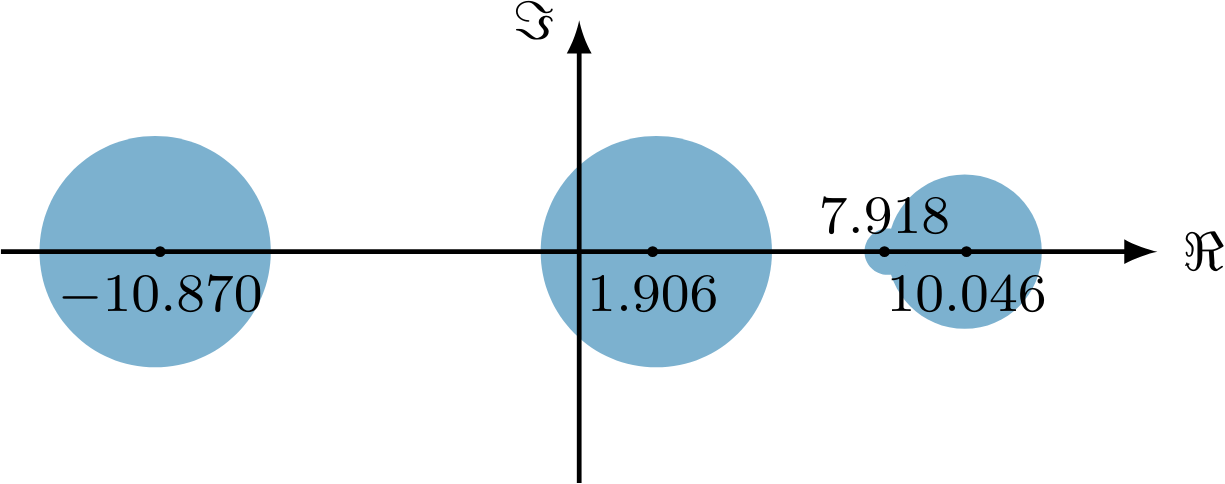
\includegraphics[width=0.4\linewidth]{./img/gershgorin.png}
        \end{figure}
    \end{example}
\end{theorem}

% \begin{lemma}
%     If all the disks are within the unit disk, the eigenvalues are stable.
%     \[
%         \begin{bmatrix}
%             \frac{1}{2} & \frac{1}{2} & 0 \\
%             \frac{1}{3} & \frac{1}{3} & \frac{1}{3} \\
%             0 & \frac{3}{4} & \frac{1}{4}
%         \end{bmatrix}
%     \]
% \end{lemma}


\begin{theorem}[Perron-Frobenius] \label{th:perron_frobenius} \marginnote{Perron-Frobenius theorem}
    Let $\A \in \R^{N \times N}$ with $N \geq 2$ be a non-negative matrix. It holds that:
    \begin{itemize}
        \item There exists a real eigenvalue $\lambda \geq 0$ that is dominant for all the other eigenvalues $\mu \in \text{spec}(\A) \smallsetminus \{\lambda\}$ (i.e., $\lambda \geq |\mu|$),
        \item The right eigenvector $\v \in \R^N$ and left eigenvector $\w \in \R^N$ associated to $\lambda$ can be chosen to be non-negative.
    \end{itemize}
    If $\A \in \R^{N \times N}$ is irreducible, then:
    \begin{itemize}
        \item The eigenvalue $\lambda$ is strictly positive ($\lambda > 0$) and simple.
        \item The right and left eigenvalues $\v$ and $\w$ associated to $\lambda$ are unique and positive.
    \end{itemize}
    If $\A \in \R^{N \times N}$ is primitive, then:
    \begin{itemize}
        \item The eigenvalue $\lambda$ is strictly dominant for all $\mu \in \text{spec}(\A) \smallsetminus \{\lambda\}$ (i.e., $\lambda > |\mu|$).
    \end{itemize}
\end{theorem}

\begin{lemma} \label{th:row_stochastic_unit_disk}
    Given a row stochastic matrix $\A$, it holds that:
    \begin{itemize}
        \item $\lambda=1$ is an eigenvalue,
        \item By \hyperref[th:gershgorin]{Gershgorin Theorem}, $\text{spec}(\A)$ is a subset of the unit disk (i.e., all Gershgorin disks lie inside the unit disk).
    \end{itemize}

    \begin{figure}[H]
        \centering
        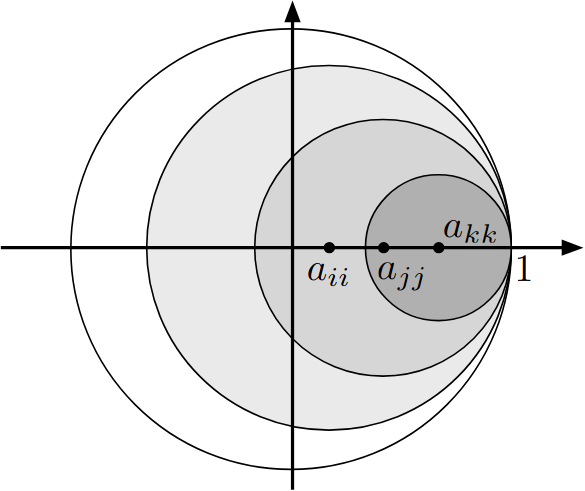
\includegraphics[width=0.2\linewidth]{./img/gershgorin_unit.png}
    \end{figure}

    \indenttbox
    \begin{corollary}
        The eigenvalue $\lambda=1 \geq |\mu|$ is dominant.
    \end{corollary}
\end{lemma}

\begin{lemma}
    Given a row stochastic and primitive matrix $\A$, by \Cref{th:row_stochastic_unit_disk} and \hyperref[th:perron_frobenius]{Perron-Frobenius Theorem} it holds that $\lambda = 1$ is simple and strictly dominant.

    \indenttbox
    \begin{corollary}
        The consensus averaging system is marginally stable (i.e., converges but not necessarily to the origin) as the largest distinct eigenvalue is $\lambda = 1$.
    \end{corollary}
\end{lemma}


% \begin{lemma}
%     \[
%         \x_\text{eq} = ker(\matr{I} - \A) = \{ \vec{1}\beta \mid \beta \in \R \}
%     \]

%     \[
%         \w^T \x^{k+1} = \w^T(\A \x^{k}) = \w^T \x^k
%     \]
%     i.e., $\w$ is left eigenvector of $\A$ with $\lambda = 1$.

%     Therefore, the above must be true for:
%     \[
%         \begin{split}
%             \w^T \x_\text{eq} \\
%             \w^T \x^{0} \\
%         \end{split}
%     \]
%     \[
%         \w^T \vec{1}\beta \Rightarrow \beta = \frac{\w^T\x^{0}}{\w^T\vec{1}}
%     \]
% \end{lemma}

\begin{theorem}[Discrete-time consensus] \marginnote{Discrete-time consensus}
    Consider a discrete-time averaging system with digraph $G$ and weighted adjacency matrix $\matr{A}$. Assume $G$ strongly connected and aperiodic, and $\matr{A}$ row stochastic. 
    
    It holds that there exists a left eigenvector $\vec{w} \in \mathbb{R}^N$, $\vec{w} > 0$ such that the consensus converges to:
        \[ 
            \lim_{k \rightarrow \infty} \vec{x}^k 
            = \vec{1}\frac{\vec{w}^T \vec{x}^0}{\vec{w}^T\vec{1}} 
            = \begin{bmatrix} 1 \\ \vdots \\ 1 \end{bmatrix} \frac{\sum_{i=1}^N w_i x_i^0}{\sum_{j=1}^N w_j}
            = \begin{bmatrix} 1 \\ \vdots \\ 1 \end{bmatrix} \sum_{i=1}^N \frac{w_i}{\sum_{j=1}^N w_j} x_i^0
        \]
        where $\tilde{w}_i = \frac{w_i}{\sum_{i=j}^N w_j}$ are all normalized and sum to 1 (i.e., they produce a convex combination).

    Moreover, if $\matr{A}$ is doubly stochastic, then it holds that the consensus is the average as $\vec{w} = 1$:
    \[ 
        \lim_{k \rightarrow \infty} \vec{x}^k = \vec{1} \frac{1}{N} \sum_{i=1}^N x_i^0
    \]

    % \begin{proof}[Sketch of proof]
    %     Let $\matr{T} = \begin{bmatrix} \vec{1} & \vec{v}^2 & \cdots & \vec{v}^N \end{bmatrix}$ be a change in coordinates that transforms an adjacency matrix into its Jordan form $\matr{J}$:
    %     \[ \matr{J} = \matr{T}^{-1} \matr{A} \matr{T} \]
    %     As $\lambda=1$ is a simple eigenvalue (\Cref{th:strongly_connected_eigenvalues}), it holds that:
    %     \[
    %         \matr{J} = \begin{bmatrix}
    %             1 & 0 & \cdots & 0 \\
    %             0 & & &  \\
    %             \vdots & & \matr{J}_2 &  \\
    %             0 & & &  \\
    %         \end{bmatrix}
    %     \]
    %     where the eigenvalues of $\matr{J}_2 \in \mathbb{R}^{(N-1) \times (N-1)}$ lie inside the open unit disk.

    %     Let $\vec{x}^k = \matr{T}\bar{\vec{x}}^k$, then we have that:
    %     \[
    %         \begin{split}
    %             &\vec{x}^{k+1} = \matr{A} \vec{x}^{k} \\
    %             &\iff \matr{T} \bar{\vec{x}}^{k+1} = \matr{A} (\matr{T} \bar{\vec{x}}^k) \\
    %             &\iff \bar{\vec{x}}^{k+1} = \matr{T}^{-1} \matr{A} (\matr{T} \bar{\vec{x}}^k) = \matr{J}\bar{\vec{x}}^k 
    %         \end{split}
    %     \]
    %     Therefore:
    %     \[
    %         \begin{gathered}
    %             \lim_{k \rightarrow \infty} \bar{\vec{x}}^k = \bar{x}_1^0 \begin{bmatrix} 1 \\ 0 \\ \vdots \\ 0 \end{bmatrix} \\
    %             \bar{x}_1^{k+1} = \bar{x}_1^k \quad \forall k \geq 0 \\
    %             \lim_{k \rightarrow \infty} \bar{x}_i^{k} = 0 \quad \forall i = 2, \dots, N \\
    %         \end{gathered}
    %     \]
    % \end{proof}

    \begin{proof}[Proof (Jordan-form approach)]
        As is $G$ strongly connected and aperiodic, and $\A$ is row stochastic, it holds that:
        \begin{itemize}
            \item By \Cref{th:positive_matrix_digraph_connected}, $\A$ is primitive.
            \item By \hyperref[th:perron_frobenius]{Perron-Frobenius Theorem} and \Cref{th:row_stochastic_unit_disk}, the eigenvalue $\lambda=1$ is strictly dominant and it is associated to the right eigenvector $\vec{1}$ (row stochasticity) and left eigenvector $\w$.
        \end{itemize}
    
        Consider the non-singular matrix $\matr{T} \in \R^{N \times N}$ defined as:
        \[
            \matr{T} = \begin{bmatrix}
                \vert & \vert & & \vert \\
                \vec{1} & \v^2 & \dots & \v^N \\
                \vert & \vert & & \vert \\
            \end{bmatrix} = \begin{bmatrix}
                \vec{1} & \matr{W}_R
            \end{bmatrix}
            \qquad
            \matr{T}^{-1} = \begin{bmatrix}
                - & (\w)^T & - \\
                - & (\w^2)^T & - \\
                - & \vdots & - \\
                - & (\w^N)^T & - \\
            \end{bmatrix} = \begin{bmatrix}
                \w^T \\ \matr{W}_L
            \end{bmatrix}
        \]
    
        A change in coordinates defined as:
        \[
            \x \mapsto \tilde{\x} = \matr{T}^{-1} \x
        \]
        allows to obtain the Jordan form $\matr{T}^{-1}\A\matr{T}$:
        \[
            \matr{T}^{-1}\A\matr{T} = \begin{bmatrix}
                1 & 0 & \dots \\
                0 & & \\
                \vdots & & \matr{J}_2 \\
            \end{bmatrix}
        \]
        with $\matr{J}_2 \in \mathbb{R}^{(N-1) \times (N-1)}$ Schur (i.e., $\text{spec}(\matr{J}_2)$ inside the open unit disk).
    
        The dynamics $\x^{k+1} = \A \x^k$ in the new coordinate system is:
        \[
            \begin{split}
                \tilde{\x}^{k+1} &= \matr{T}^{-1} \x^{k+1} = \matr{T}^{-1} \A \matr{T} \tilde{\x}^k \\
                &= \begin{bmatrix}
                    1 & 0 & \dots \\
                    0 & & \\
                    \vdots & & \matr{J}_2 \\
                \end{bmatrix} \tilde{\x}^k
                = \begin{bmatrix}
                    1 & 0 & \dots \\
                    0 & & \\
                    \vdots & & \matr{J}_2 \\
                \end{bmatrix}^{k+1} \tilde{\x}^0
            \end{split}
        \]
        Let's denote:
        \[
            \tilde{\x}^k = \matr{T}^{-1}\x^k = \begin{bmatrix}
                \w^T\x^k \\ \matr{W}_L\x^k
            \end{bmatrix}
            = \begin{bmatrix}
                \tilde{\x}^k_{m} \\ \tilde{\x}^k_{\bot}
            \end{bmatrix}
        \]
        We have that:
        \[
            \begin{split}
                \lim_{k \rightarrow \infty} \tilde{\x}^k
                &= \lim_{k \rightarrow \infty} \begin{bmatrix}
                    1 & 0 & \dots \\
                    0 & & \\
                    \vdots & & \matr{J}_2 \\
                \end{bmatrix}^k \tilde{\x}^0 \\
                &= \lim_{k \rightarrow \infty} \begin{bmatrix}
                    1 & 0 & \dots \\
                    0 & & \\
                    \vdots & & (\matr{J}_2)^k \\
                \end{bmatrix} \begin{bmatrix}
                    \tilde{\x}^0_{m} \\ \tilde{\x}^0_{\bot}
                \end{bmatrix} \\
                &= \begin{bmatrix}
                    1 \cdot \tilde{\x}^0_{m} \\ 
                    \lim_{k \rightarrow \infty} (\matr{J}_2)^k \tilde{\x}^0_{\bot}
                \end{bmatrix} \\
                &= \begin{bmatrix}
                    \w^T \x^0 \\ 
                    0
                \end{bmatrix} \\
            \end{split}
        \]
        Note that $\lim_{k \rightarrow \infty} \matr{J}_2^k = 0$ as it is stable (i.e., all eigenvalues are in the open unit disk $|\mu| < 1$).
    
        In the original coordinate system, the limit is:
        \[
            \begin{split}
                \lim_{k \rightarrow \infty} \x^k 
                &= \lim_{k \rightarrow \infty} \matr{T} \tilde{\x}^k \\
                &= \matr{T} \lim_{k \rightarrow \infty} \tilde{\x}^k \\
                &= \begin{bmatrix}
                    \vec{1} & \matr{W}_R
                \end{bmatrix} \begin{bmatrix}
                    \w^T \x^0 \\ 
                    0
                \end{bmatrix} 
                = \vec{1} (\w^T \x^0)
            \end{split}
        \]
        
        \indenttbox
        \begin{remark}
            It is assumed that $\Vert \w \Vert = 1$ (i.e., no normalization term).
        \end{remark}
    \end{proof}

    % \begin{proof}[Lyapunov approach]
    %     $\A - \vec{1}\w^T$ is rank-1. This is to change one specific eigenvalue (move 1 to 0).

    %     Dissensus vector represents error:
    %     \[
    %         \begin{split}
    %             delta^{k+1} 
    %             = \x^{k+1} - \vec{1}\w^T \x^0 \\
    %             = \x^{k+1} - \vec{1}\w^T \x^{k+1} \\
    %             = (\matr{I} - \vec{1}\w^T) \x^{k+1} \\
    %             = (\matr{I} - \vec{1}\w^T) \A\x^{k} \\
    %             = (\A - \vec{1}\w^T) \x^{k} \\
    %             = (\A - \vec{1}\w^T) \delta^{k} \\
    %         \end{split}
    %     \]

    %     Study:
    %     \[
    %         \delta^{k+1} = (\A - \vec{1}\w^T) \delta{k}
    %     \]
    %     If $\delta^k \rightarrow 0$, then $\x^k \rightarrow\vec{1}\w^T\x^0$.
    %     Note $(\A - \vec{1}\w^T)$ is Schur.

    %     Lyapunov equation for discrete time systems:
    %     \[
    %         \bar{\A}^T \matr{P} \bar{\A} = - \matr{P} = - \matr{Q}
    %     \]
    %     where $\bar{\A}$ is the Jordan-form of $(\A - \vec{1}\w^T)$

    %     Select $Q_2$ to be block-diagonal and $p_1$


    %     \[
    %         V(\delta) = \delta^T (\matr{T}^{-1})^T \matr{P} \matr{T}^{-1} \delta
    %     \]
    % \end{proof}
\end{theorem}

\end{subappendices}